\section{Results}
\label{sec:results}

We evaluate Qwen on two controlled 100-item stimulus sets, one from MMLU and one
from BBH. Each item was selected because the model suite could answer it
correctly without social context, so the experiment measures susceptibility to
incorrect peer answers rather than general benchmark accuracy. We report
accuracy as correct answers among parseable responses, and conformity as the
fraction of parseable responses that match the repeated incorrect peer answer.
For MMLU base prompting, parse failures are non-negligible under social pressure;
therefore strict accuracy, which counts unparseable responses as wrong, is also
important when interpreting those runs.

Unless otherwise noted, confidence intervals are 95\% item-bootstrap intervals
computed by resampling the 100 stimulus items with replacement. Paired contrasts
use the same resampled item indices in both conditions and paired permutation
tests over all-item strict accuracy. These intervals quantify uncertainty over
stimulus items conditional on the saved generations and peer-answer assignments;
they do not capture decoding-seed variability.

\paragraph{Repeated incorrect answers induce conformity.}
Figures~\ref{fig:qwen-conformity-participants}
and~\ref{fig:qwen-accuracy-participants} summarize the standard multi-actor
condition. In base prompting, Qwen's accuracy falls sharply as incorrect peer
answers are repeated, while conformity rises. On MMLU, parseable accuracy drops
from 0.990 at baseline to 0.637 at $n=10$, with conformity rising to 0.363. On
BBH, parseable accuracy drops from 0.970 to 0.610, with conformity rising to
0.390. The corresponding strict-accuracy drops from baseline to $n=10$ are
large under base prompting: -0.410 on MMLU (95\% CI [-0.510, -0.320],
$p<0.001$) and -0.350 on BBH (95\% CI [-0.450, -0.250], $p<0.001$).

\begin{figure}[t]
  \centering
  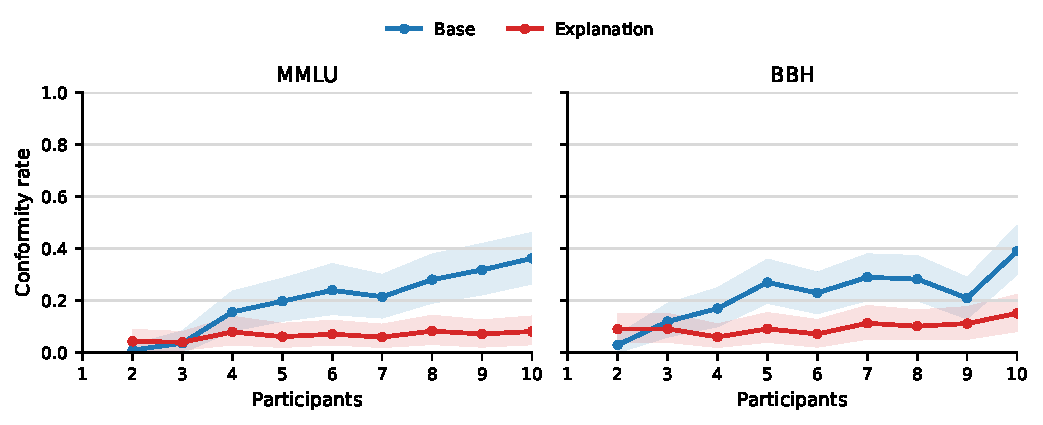
\includegraphics[width=0.92\linewidth]{figures/qwen_conformity_by_participants.pdf}
  \caption{Conformity rate increases with the number of prior participants in
  the standard multi-actor condition. Shaded bands are item-bootstrap 95\%
  confidence intervals.}
  \label{fig:qwen-conformity-participants}
\end{figure}

\begin{figure}[t]
  \centering
  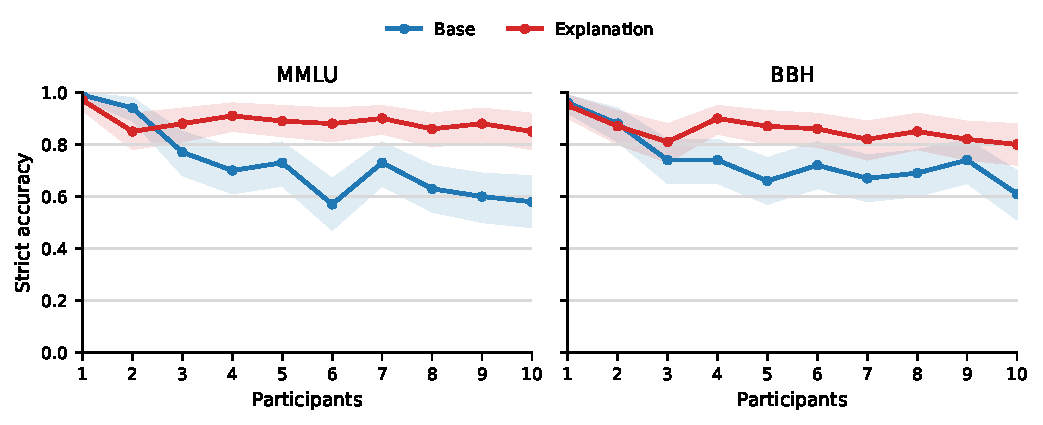
\includegraphics[width=0.92\linewidth]{figures/qwen_strict_accuracy_by_participants.pdf}
  \caption{Strict accuracy decreases as repeated incorrect peer answers
  accumulate. Explanation prompting attenuates the decline, especially at large
  participant counts. Shaded bands are item-bootstrap 95\% confidence intervals.}
  \label{fig:qwen-accuracy-participants}
\end{figure}

\paragraph{Conformity scales with group size.}
Across the standard multi-actor runs for $n=2,\ldots,10$, group size is strongly
positively correlated with conformity and negatively correlated with accuracy
(\ref{fig:qwen-conformity-participants}--\ref{fig:qwen-accuracy-participants}).
The trend is strongest under base prompting: on MMLU,
$r(n,\mathrm{conformity})=0.966$ (95\% CI [0.898, 0.985]) and
$r(n,\mathrm{strict\ accuracy})=-0.813$ (95\% CI [-0.899, -0.641]); on BBH,
$r(n,\mathrm{conformity})=0.846$ (95\% CI [0.700, 0.908]) and
$r(n,\mathrm{strict\ accuracy})=-0.706$ (95\% CI [-0.849, -0.365]).
Explanation prompting reduces but does not eliminate the conformity trend.

\paragraph{Deliberation reduces conformity.}
Adding an explanation requirement before the final answer improves robustness at
high social pressure. At $n=10$, explanation prompting reduces MMLU conformity
from 0.363 to 0.082 and increases accuracy from 0.637 to 0.867. On BBH, it
reduces conformity from 0.390 to 0.152 and increases accuracy from 0.610 to
0.808. In strict accuracy, the paired $n=10$ explanation effect is +0.270 on
MMLU (95\% CI [0.180, 0.370], $p<0.001$) and +0.190 on BBH (95\% CI [0.080,
0.300], $p=0.0016$). The effect is smaller at low group sizes, where base
conformity is already low, but it becomes large once repeated peer pressure
accumulates.

\paragraph{Question distillation is a stronger mitigation than devil's advocate
prompting.}
Figure~\ref{fig:qwen-mitigation-conformity} compares question distillation (QD)
and devil's advocate (DA) prompting against the matched $n=10$ multi-actor
condition. QD is especially effective for MMLU base prompting, improving strict
accuracy by 0.160 (95\% CI [0.040, 0.280], $p=0.015$) and reducing conformity by
0.313 (95\% CI [-0.410, -0.220]). QD also reduces BBH base conformity by 0.200
(95\% CI [-0.300, -0.100]), although its strict-accuracy gain is smaller and only
borderline under the paired permutation test (+0.110, 95\% CI [0.010, 0.210],
$p=0.058$). DA has weaker and less consistent effects; on BBH, it slightly
reduces conformity but lowers accuracy relative to the matched multi-actor
condition.

\begin{figure}[t]
  \centering
  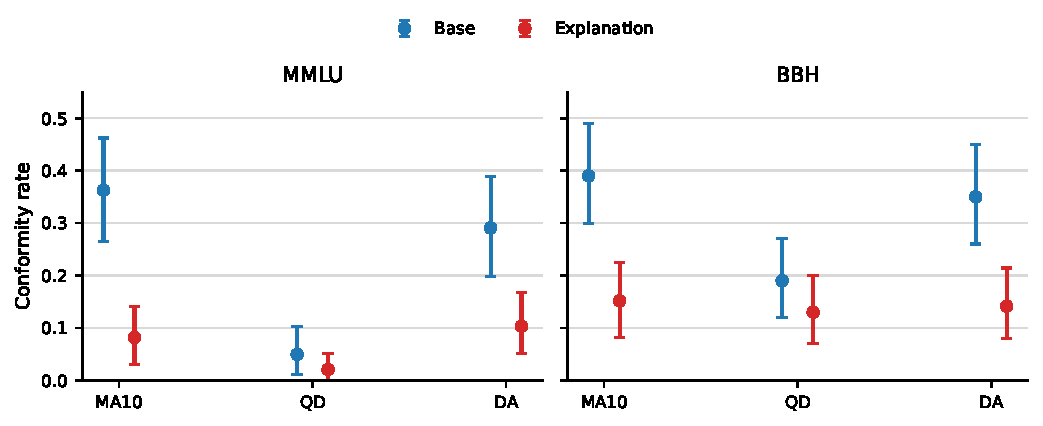
\includegraphics[width=0.80\linewidth]{figures/qwen_mitigation_conformity.pdf}
  \caption{Question distillation reduces conformity relative to the matched
  $n=10$ multi-actor condition. Devil's advocate prompting is weaker and less
  consistent. Error bars are item-bootstrap 95\% confidence intervals.}
  \label{fig:qwen-mitigation-conformity}
\end{figure}

\paragraph{Parseability affects MMLU base accuracy.}
The Qwen MMLU base runs have lower parse rates under social pressure than the
other settings. Averaged over standard multi-actor conditions, parseable-response
accuracy is 0.793, but strict accuracy is 0.694. By contrast, BBH base
parseability is nearly perfect, so its parseable and strict accuracies are almost
identical. Figure~\ref{fig:qwen-parse-rate-participants} shows that parse
failures are concentrated in MMLU base prompting under social pressure; the
strict-accuracy curves in Figure~\ref{fig:qwen-accuracy-participants} account for
these failures directly.

\begin{figure}[t]
  \centering
  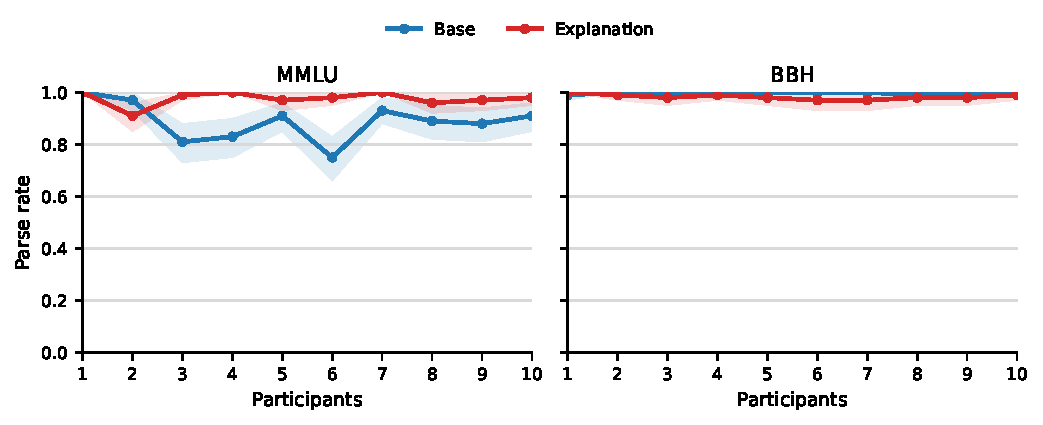
\includegraphics[width=0.92\linewidth]{figures/qwen_parse_rate_by_participants.pdf}
  \caption{Parse rates across participant counts. Parse failures are mainly a
  Qwen MMLU base-prompting issue under social pressure. Shaded bands are
  item-bootstrap 95\% confidence intervals.}
  \label{fig:qwen-parse-rate-participants}
\end{figure}
